\documentclass[11pt]{article}

\usepackage{float}
\usepackage{hyperref}
\usepackage{graphicx}
% formatting
\usepackage{verbatim}
\usepackage{moreverb}
\usepackage{minted}
\usepackage{parskip}
\usepackage{amsmath}
\usepackage[listings]{tcolorbox}
\usepackage{enumerate}
\usepackage{tikz}
\usetikzlibrary{arrows,automata, positioning}
\let\verbatiminput=\verbatimtabinput
\def\verbatimtabsize{4\relax}

\newcommand{\RepoRootPath}{fpga\_labs\_fa19}

\tcbset{
texexp/.style={colframe=black, colback=lightgray!15,
         coltitle=white,
         fonttitle=\small\sffamily\bfseries, fontupper=\small, fontlower=\small},
     example/.style 2 args={texexp,
title={Question \thetcbcounter: #1},label={#2}},
}

\newtcolorbox{texexp}[1]{texexp}
\newtcolorbox[auto counter]{texexptitled}[3][]{%
example={#2}{#3},#1}

\setlength{\topmargin}{-0.5in}
\setlength{\textheight}{9in}
\setlength{\oddsidemargin}{0in}
\setlength{\evensidemargin}{0in}
\setlength{\textwidth}{6.5in}

% Useful macros

\newcommand{\note}[1]{{\bf [ NOTE: #1 ]}}
\newcommand{\fixme}[1]{{\bf [ FIXME: #1 ]}}
\newcommand{\wunits}[2]{\mbox{#1\,#2}}
\newcommand{\um}{\mbox{$\mu$m}}
\newcommand{\xum}[1]{\wunits{#1}{\um}}
\newcommand{\by}[2]{\mbox{#1$\times$#2}}
\newcommand{\byby}[3]{\mbox{#1$\times$#2$\times$#3}}


\newenvironment{tightlist}
{\begin{itemize}
 \setlength{\parsep}{0pt}
 \setlength{\itemsep}{-2pt}}
{\end{itemize}}

\newenvironment{titledtightlist}[1]
{\noindent
 ~~\textbf{#1}
 \begin{itemize}
 \setlength{\parsep}{0pt}
 \setlength{\itemsep}{-2pt}}
{\end{itemize}}

% Change spacing before and after section headers

\makeatletter
\renewcommand{\section}
{\@startsection {section}{1}{0pt}
 {-2ex}
 {1ex}
 {\bfseries\Large}}
\makeatother

\makeatletter
\renewcommand{\subsection}
{\@startsection {subsection}{1}{0pt}
 {-1ex}
 {0.5ex}
 {\bfseries\normalsize}}
\makeatother

% Reduce likelihood of a single line at the top/bottom of page
\clubpenalty=2000
\widowpenalty=2000

% Other commands and parameters
\pagestyle{myheadings}
\setlength{\parindent}{0in}
\setlength{\parskip}{10pt}

% Commands for register format figures.
\newcommand{\instbit}[1]{\mbox{\scriptsize #1}}
\newcommand{\instbitrange}[2]{\instbit{#1} \hfill \instbit{#2}}

% Break lines on texttt text on underscores
% See: https://tex.stackexchange.com/questions/315369/how-to-deal-with-bad-line-wrapping-of-texttt
\newcommand*\ttvar[1]{\texttt{\expandafter\dottvar\detokenize{#1}\relax}}
\newcommand*\dottvar[1]{\ifx\relax#1\else
  \expandafter\ifx\string_#1\string_\allowbreak\else#1\fi
  \expandafter\dottvar\fi}

\begin{document}

\def\PYZsq{\textquotesingle}
\title{\vspace{-0.4in}\Large \bf EECS 151/251A FPGA Lab 5:\\FSMs and UART \vspace{-0.1in}}

\author{Prof. Borivoje Nikolic and Prof. Sophia Shao \\
TAs: Cem Yalcin, Rebekah Zhao, Ryan Kaveh, Vighnesh Iyer \\ Department of Electrical Engineering and Computer Sciences\\
College of Engineering, University of California, Berkeley}
\date{}
\maketitle

\newcommand{\headertext}{EECS 151/251A FPGA Lab 5: FSMs and UART}
\markboth{\headertext}{\headertext}
\thispagestyle{empty}

\section{Before You Start This Lab}
Run \verb|git pull| in \texttt{\RepoRootPath}.
Copy the modules you created in the previous lab to this lab:
\begin{minted}{text}
  cd fpga_labs_fa19
  cp lab4/src/synchronizer.v lab5/src/.
  cp lab4/src/debouncer.v lab5/src/.
  cp lab4/src/edge_detector.v lab5/src/.
  cp lab4/src/tone_generator.v lab5/src/.
  cp lab4/src/music_streamer.v lab5/src/.
\end{minted}

Review these documents:
\begin{enumerate}
  \item \href{http://inst.eecs.berkeley.edu/~eecs151/fa19/files/verilog/verilog_fsm.pdf}{verilog\_fsm.pdf} - constructing FSMs in Verilog.
  \item \href{http://inst.eecs.berkeley.edu/~eecs151/fa19/files/verilog/ready_valid_interface.pdf}{ready\_valid.pdf} - ready/valid interfaces and handshakes. Try drawing out the timing diagrams for the ready/valid handshake before trying to write any Verilog for the UART.
\end{enumerate}

In the first part of this lab, you will extend the \verb|music_streamer| from lab 4 to implement a simple FSM.
Then you will implement a UART (Universal Asynchronous Receiver / Transmitter) device, otherwise known as a serial interface.
Your working UART from this lab will be used in your project to talk to your workstation (desktop) over a serial line.

\section{Music Streamer FSM}
Implement a simple FSM in the \verb|music_streamer|.

The FSM has 3 states: \verb|PAUSED|, \verb|REGULAR_PLAY|, \verb|REVERSE_PLAY|.
Here is the state transition diagram:
\begin{center}
\begin{tikzpicture}[shorten >=1pt, node distance=10cm,on grid, auto,line width=0.05cm]
  \tikzstyle{state} = [draw, very thick, fill=white, rectangle, minimum height=3em, minimum width=7em, node distance=17em, font={\sffamily\bfseries}]
  \tikzstyle{stateEdgePortion} = [black,thick];
  \tikzstyle{stateEdge} = [stateEdgePortion,->,line width=3cm];
  \tikzstyle{edgeLabel} = [pos=0.5, text centered, font={\sffamily\small}];

  \node[state,initial](rp) {REGULAR\_PLAY};
  \node[state](revp) [below =of rp]{REVERSE\_PLAY};
  \node[state](p) [right=of rp]{PAUSED};

  \path[->]
  (rp) edge node {Play-pause button} (p)
    edge [swap] node {Reverse button} (revp)
    edge [loop above] node {} (rp)
  (p) edge node {} (rp)
    edge [loop below] node {} (p)
  (revp) edge [swap] node {Play-pause button} (p)
    edge [swap] node {} (rp)
    edge [loop below] node {} (revp);
\end{tikzpicture}
\end{center}

\begin{enumerate}
  \item The initial state should be \verb|REGULAR_PLAY|.
  \item Pressing the \verb|play_pause| button should transition you into the \verb|PAUSED| state from either the \verb|REGULAR_PLAY| or \verb|REVERSE_PLAY| states. Pressing the same button while in the \verb|PAUSED| state should transition the FSM to the \verb|REGULAR_PLAY| state.
  \item In the \verb|PAUSED| state, the ROM address should be held steady at its value before the transition into \verb|PAUSED| and no sound should come out of the speaker. After leaving the \verb|PAUSED| state the ROM address should begin incrementing again from where it left off and the speaker should play the tones.
  \item You can toggle between the \verb|REGULAR_PLAY| and \verb|REVERSE_PLAY| states by using the \verb|reverse| button. In the \verb|REVERSE_PLAY| state you should decrement the ROM address by 1 rather than incrementing it by 1 every X clock cycles as defined by the tempo.
  \item If you don't press any buttons, the FSM shouldn't transition to another state.
\end{enumerate}

The \verb|music_streamer| takes in user button inputs (\verb|play_pause, reverse|) that it can use to transition states.

Also, drive the LEDs so that they show the current state as such:
\renewcommand{\arraystretch}{1.5}
\begin{center}
\begin{tabular}{| l | l |}
  \hline
  \textbf{LED} & \textbf{Value} \\ \hline
      leds[0] & \verb|current_state| == \verb|REGULAR_PLAY| \\ \hline
      leds[1] & \verb|current_state| == \verb|PAUSED| \\ \hline
      leds[2] & \verb|current_state| == \verb|REVERSE_PLAY| \\ \hline
\end{tabular}
\end{center}

Look at the commented code in \ttvar{music_streamer_testbench.v} that tests the state machine.
Uncomment and run the test and inspect the waveform to check that the FSM is performing correctly.

Next, modify \verb|z1top.v| to connect the \verb|play_pause| and \verb|reverse| ports to \verb|buttons_pressed| [2] and [3] respectively, and the bottom 4 bits of \verb|LEDS| to the \verb|leds| output of the \verb|music_streamer|.
You should copy your \textit{implementation} of \verb|z1top.v| from lab 4, but leave the top-level IOs in the skeleton untouched.

Finally, program the FPGA with the \verb|music_streamer|, and verify its functionality.

\section{Serial Device}
You are responsible only for implementing the \textbf{transmit} side of the UART for this lab. As you should have inferred from reading the ready/valid tutorial, the UART transmit and receive modules use a ready/valid interface to communicate with other modules on the FPGA.

Both the UART’s receive and transmit modules will have their own separate set of ready/valid interfaces connected appropriately to external modules.

Please note that the serial line itself is not a ready/valid interface. Rather, it is the modules you will work with in this lab (\verb|uart_transmitter| and \verb|uart_receiver|) that have the ready/valid handshake for interfacing with other modules on the FPGA.

\subsection{Framing}
On the \verb|Pynq-Z1| board, the physical signaling aspects (such as voltage level) of the serial connection will be taken care of by off-FPGA devices. From the FPGA's perspective, there are two signals, \verb|FPGA_SERIAL_RX| and \verb|FPGA_SERIAL_TX|, which correspond to the receive-side and transmit-side pins of the serial port. The FPGA's job is to correctly frame characters going back and forth across the serial connection. Figure 1 below shows a single character frame being transmitted and will be extremely useful in understanding the protocol.

\begin{figure}[H]
  \centerline{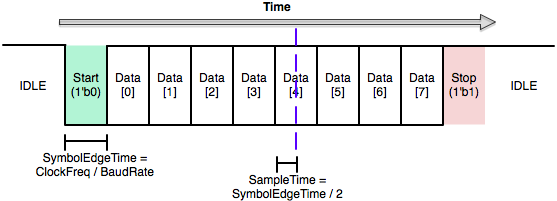
\includegraphics[width=6in]{figs/uart_frame.png}}
  \caption{UART Frame Structure}
\end{figure}

In the idle state the serial line is held high. When the TX side is ready to send a character, it pulls the line low. This is called the start bit. Because UART is an asynchronous protocol, all timing within the frame is relative to when the start bit is first sent (or detected, on the receive side).

The frame is divided up in to 10 uniformly sized bits: the start bit, 8 data bits, and then the stop bit. The width of a bit in cycles of the system clock is then naturally given by the system clock frequency divided by the baudrate. The baudrate is the number of bits sent per second; in this lab the baudrate will be 115200. Notice that both sides must agree on a baudrate for this scheme to be feasible.

\subsection{Transmitting}
Let us first think about sending a character using this scheme. Once we have a character that we want to send out, transmitting it is simply a matter of shifting each bit of the character, plus the start and stop bits, out of a shift register on to the serial line.

Remember, the serial baudrate is much slower than the system clock, so we must wait $SymbolEdgeTime = \frac{ClockFreq}{BaudRate}$ cycles between changing the character we're putting on the serial line. After we have shifted all 10 bits out of the shift register, we are done unless we see another transmission immediately after.

\subsection{Receiving}
The receive side is a bit more complicated. Fortunately, we will provide the receiver module. Open \verb|lab5/lab5.srcs/sources_1/new/uart_receiver.v| so you can see the explanation below implemented.

Like the transmit side, the receive side of the serial device is essentially just a shift register, but this time we are shifting bits from the serial line into the shift register. However, care must be taken into determining when to shift bits in. If we attempt to sample the serial signal directly on the edge between two symbols, we are exceedingly likely to sample on the wrong side of the edge (or worse, when the signal is transitioning) and get the wrong value for that bit. The correct solution is to wait halfway into a cycle (until \verb|SampleTime| on the diagram) before reading a bit in to the shift register.

One other subtlety of the receive side is correctly implementing the ready/valid interface. Once we have received a full character over the serial port, we want to hold the valid signal high until the ready signal goes high, after which the valid signal will be driven low until we receive another character.

This requires using an extra flip-flop (the \verb|has_byte| reg in \verb|uart_receiver.v|) that is set when the last character is shifted in to the shift register and cleared when the ready signal is asserted. This allows us to correctly implement the ready/valid handshake.

\subsection{Putting It All Together}
Although the receive side and transmit side of the UART you will be building are essentially orthogonal, we are packaging them into one UART module to keep things tidy.
% If you look at \verb|uart.v|, you will see that this module consists of instantiations of \verb|uart_receiver| and \verb|uart_transmitter|, but there are also two \verb|iob| registers that the serial lines are fed through. What are these for? The \verb|iob| directive tells the synthesis tool to pack those registers into a special block called an \verb|IOB|, which is used to drive and sense from the IO pins. Using an \verb|IOB| helps ensure that you will have a nice, clean, well-behaved off-chip signal to use as an input or output to your serial modules.
The diagram below shows the entire setup:
\begin{figure}[H]
  \centerline{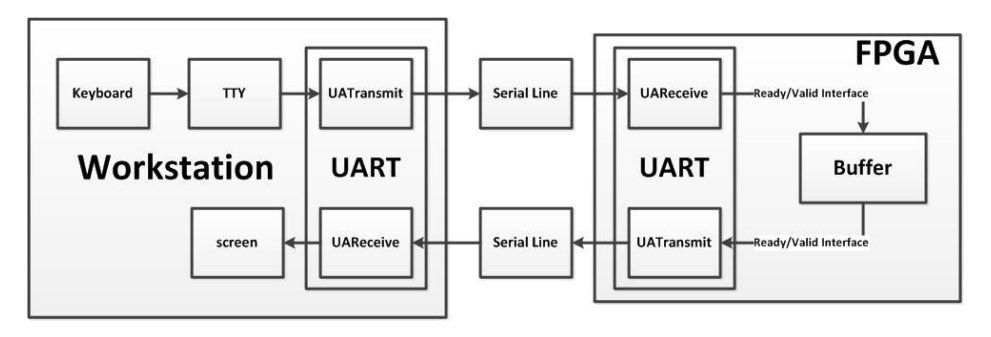
\includegraphics[width=6in]{figs/high_level_diagram.png}}
  \caption{High Level Diagram}
\end{figure}

\subsection{Simulation}
We have provided a simple testbench, called \verb|uart_testbench| that will run some basic tests on two instantiations of the UART module with their RX and TX signals crossed so that they can talk to each other. There is also a \verb|.do| file that will run the test. You should note that this test bench reporting success is \textbf{not} by itself a good indication that your UART is working properly. The testbench does not attempt to test back to back UART transmissions so you will have to add that test in yourself. Due to the way x's are treated by Modelsim if many signals in your design are undefined the testbench may erroneously pass. Make sure to look at the waveform to see that everything appears to be working properly and that you adequately purge your simulation of high Z and undefined X signals.

If the testbench prints out \verb|# <EOF>| it means that it timed out; this indicates that the testbench was stuck waiting for a condition that never became true. Inspect the waveform and match it up to the testbench code to see where it hangs and why. You shouldn't need to increase any of the timeouts in the \verb|.do| files.

\section{Echo}

Your UART will eventually be used to interact with your CPU from your workstation. However, since you don't have a CPU yet, you need some other way to test that your UART works on the board.

We have provided this for you. The provided \verb|z1top| contains a very simple finite state machine that does the following continuously:

\begin{itemize}
  \item Pulls a received character from the \verb|uart_receiver| using ready/valid
  \item If the received character is an ASCII letter (A-Z or a-z), its case is inverted (lower to upper case or upper or lower case)
  \item If the received character isn't an ASCII letter, it is unmodified
  \item The possibly modified character is sent to the \verb|uart_transmitter| using ready/valid to be sent over the serial line one bit at a time
\end{itemize}

Check using the provided \verb|echo_testbench.v| testbench that everything works as it should in simulation. This testbench is heavily commented to help you understand the communication between the 2 UARTs and the communication over the ready/valid interface. The file often refers to the UART on the workstation as the off-chip UART and the UART on the FPGA as the on-chip UART.

\subsection{PMOD serial interface}

The Pynq-Z1 does not have an RS-232 serial interface! Well, ok, it does, kind of. The USB interface you use for programming the board (and for RS-232 communication with the board's ARM-based system) is actually only connected to the Processor Subsystem, not the Programmable Logic. We can't use it from our design directly. So, we need to add a serial interface: this is usually a chip wired to connect a device as a serial host/client to another device, with appropriate voltage level shifting to meet the electrical specification (e.g. RS-232). Before you can continue, therefore, you must upgrade your Pynq-Z1 with one: the \href{https://store.digilentinc.com/pmod-usbuart-usb-to-uart-interface/}{Pmod USBUART} is available for you in this lab. (The \href{https://store.digilentinc.com/pmod-rs232-serial-converter-and-interface-standard/}{Pmod RS232} is another module you could use, but it doesn't take care of framing your data in the USB protocol for you.)

Have a read over the \href{https://reference.digilentinc.com/reference/pmod/pmodusbuart/reference-manual}{Pmod USBUART Reference Manual} (\verb|resources/pmodusbuart_rm.pdf|). You might agree that mapping the pin on the Zynq chip to a PMOD port, then to the right pin on the PMOD header, then to the right pin on the transceiver chip, can be quite confusing. See if you can work it out. Here's a little help:

\begin{itemize}
  \item Connect \verb|FPGA_SERIAL_TX| in your design to the Pmod USBUART's \verb|RXD| pin (PMOD header pin 2).
  \item Connect \verb|FPGA_SERIAL_RX| in your design to the Pmod USBUART's \verb|TXD| pin (PMOD header pin 3).
\end{itemize}

\textbf{What do RTS and CTS do?} Respectively \underline{R}equest to \underline{S}end and \underline{C}lear to \underline{S}end, these signals are used for hardware flow control. We will ignore them, so make sure to disable hardware flow control in the software you use to connect to your board (or more likely, make sure not to enable it by accident).

\textbf{Note:} Make sure that the power selection jumper on the Pmod USBUART is set to LCL3V3 - as you'll read in the reference manual, this is because we're powered the system from an external source and \emph{not} through the tiny USB interface chip on the PMOD module.

\subsection{Implement your design}

Synthesize your design and generate the bitstream, then program the board just like you have done in previous labs.

\textbf{Pay attention to the warnings} generated by the tool chain. Again, it's possible to write your Verilog in such a way that it passes behavioural simulation but doesn't work in implementation. Warnings about ``multi driven nets'', for example, can mean that certain logic pathways are never implemented on chip.

If you get stuck, it will help to structure your Verilog as a state machine in a very similar way to the provided \verb|uart_receiver.v|.

\subsection{Hello, world!}

Now, make sure the USB serial cable is plugged in between the Pynq-Z1 board and your workstation and then run:

\begin{minted}{bash}
screen $SERIALTTY 115200
\end{minted}

This tells \verb|screen|, a highly versatile terminal emulator, to open up the serial device with a baud rate of 115200 (you might have to run as \verb|root|). When you type a character into the terminal, it is sent to the FPGA over the \verb|FPGA_SERIAL_RX| line, encoded in ASCII. The state machine in \verb|z1top| may modify the character you sent it and will then push a new character over the \verb|FPGA_SERIAL_TX| line to your workstation. When \verb|screen| receives a character, it will display it in the terminal.

You can find which \verb|$SERIALTTY| to connect to by perusing the output of the \verb|dmesg| command (in Linux) or checking the Device Manager (in Windows).

Now, if you have a properly working design, you should be able to tap a few characters into the terminal and have them echoed to you (with inverted case if you type letters). Make sure that if you type really fast that all characters still display properly. If you see some weird garbage symbols then the data is getting corrupted and something is likely wrong. If you see this happening very infrequently, don't just hope that it won't happen while the TA is doing the checkoff; take the time now to figure out what is wrong. UART bugs are a common source of headaches for groups during the first project checkpoint.

To close \verb|screen|, type \verb|Ctrl-a| then \verb|Shift-k| and answer \verb|y| to the confirmation prompt. If you don't close screen properly, other students won't be able to access the serial port. If you try opening \verb|screen| and it terminates after a few seconds with an error saying ``Sorry, can't find a PTY'' or ``Device is busy'', execute the command \verb|killscreen| which will kill all open screen sessions that other students may have left open. Then run \verb|screen| again.

Use \verb|screen -r| to re-attach to a non-terminated screen session. You can also reboot the computer to clear all active \verb|screen| sessions.

\subsection{Checkoff}
\begin{enumerate}
    \item Walk your TA through the simulation results and show that your UART behaves as expected.
    \item Show your TA that you can successfully type characters on the keyboard and have them echoed back to display on your \verb|screen| session.
    \item Demonstrate to your TA that your I\textsuperscript{2}S clocks waveforms match the requirements in the reference manual.
\end{enumerate}

\section{Checkoff}
\begin{enumerate}
  \item Show the RTL for the input conditioning circuits and music streamer
  \item Play an audio file generated from a simulation
  \item Demonstrate the music streamer on the FPGA (FSM, tempo control, reset)
\end{enumerate}

\subsection{Lab Report}
Submit a short report containing the waveform screenshots to answer the questions in the lab.

\section*{Ackowlegement}
This lab is the result of the work of many EECS151/251 GSIs over the years including:
\begin{itemize}
\item Sp12: James Parker, Daiwei Li, Shaoyi Cheng
\item Sp13: Shaoyi Cheng, Vincent Lee
\item Fa14: Simon Scott, Ian Juch
\item Fa15: James Martin
\item Fa16: Vighnesh Iyer
\item Fa17: George Alexandrov, Vighnesh Iyer, Nathan Narevsky
\item Sp18: Arya Reais-Parsi, Taehwan Kim
\item Fa18: Ali Moin, George Alexandrov, Andy Zhou
\end{itemize}

\end{document}
